\documentclass[11pt]{article}

\usepackage[margin=1.1in]{geometry}
\usepackage{amsmath, amssymb}
\usepackage{microtype}
\usepackage{setspace}
\usepackage{booktabs}
\usepackage{graphicx}
\usepackage{hyperref}
\usepackage{natbib}

\hypersetup{colorlinks=true, linkcolor=black, citecolor=black, urlcolor=blue}

\onehalfspacing

\title{\textbf{Network Uncertainty at the Resolution of the Data}\\[0.4em]
\large Observation Grain, Reporting Clock, and Regularization\\
in Agent-Based SIR Models}

\author{John S. Schuler\\
\small Department of Computational and Data Sciences, George Mason University}

\date{CSSSA 2026 Extended Abstract}

\begin{document}

\maketitle

\begin{abstract}
\noindent
Pandemic transmission depends on contact network structure. The mean-field ODE SIR
model is therefore strictly misspecified as a mechanistic account: the $SI/N$ term
encodes uniform mixing, not actual contact topology. But misspecification alone does
does not determine how uncertain inference about the network mechanism should be.
The central question is how the observation process---the grain at which infections
are measured and the clock at which they are reported---changes the uncertainty
that remains over network structure.

We treat the network as an uncertain object and compare posterior uncertainty under
contact-network, group-level incidence, and aggregate incidence observations. Direct
contact observation sharply constrains community structure; incidence-only schemes
leave substantial uncertainty, with group grain more informative than aggregate
grain and finer aggregate timing insufficient by itself. Half-normal, exponential,
and spike-and-slab priors over the community parameter expose the central tradeoff:
shrinkage toward uniform networks prevents unsupported structural claims but accepts
conservative bias when observations cannot justify heterogeneity. As a cautionary reduction,
we also calibrate a mean-field ODE to weekly aggregate observations. Its posterior
concentrates near a pseudo-true
parameter that absorbs network structure into a lower effective aggregate rate,
understating the density-matched mean-field reference by 8.5\% in our baseline experiment.
Collecting more independent outbreaks at the same grain and clock reduces posterior
width fourfold without reducing bias. More data make the wrong model more certain
when the additional data are collected under the same insufficient observation process.
We connect this to PAC-Bayesian regularization: the ABM supplies a distribution over
heterogeneous networks, while grain and clock determine how far observation can move
that distribution away from its regularizing prior.
\end{abstract}

\section{Calibration Requires an Observation Model}

ABMs generate rich latent trajectories, but calibration data are usually coarser
\citep{epstein2008}. We therefore treat an ABM as a generative statistical model:
\[
\text{simulator} \;\to\; \text{latent social process} \;\to\; \text{observation process} \;\to\; \text{data.}
\]
The simulator encodes interaction; the observation process encodes what is measured.
\emph{Grain} is the level observed---edges, individual events, groups, or population
totals. \emph{Clock} is the reporting interval---event time, daily, weekly, or
monthly. These define different calibration problems, not merely datasets of
different quality. Our inferential target is therefore a distribution over network
parameters conditional on a specified grain and clock.

\section{Mean-Field and Network SIR}

The standard mean-field ODE SIR model \citep{kermack1927, keeling2008} is:
\[
\frac{dS}{dt} = -\beta_{ODE}\frac{SI}{N}, \qquad
\frac{dI}{dt} = \beta_{ODE}\frac{SI}{N} - \gamma I, \qquad
\frac{dR}{dt} = \gamma I.
\]
The product $SI/N$ encodes uniform mixing: it is a social assumption, not merely
algebra. A network SIR instead gives susceptible agent $i$ infection probability
\citep{keeling2008,kiss2017}
\[
P\!\bigl(i \text{ infected in } [t,\,t+\Delta t]\bigr)
= 1 - \exp\!\Bigl(-\beta\,\Delta t \sum_{j \in \mathcal{N}(i)} \mathbf{1}\{X_j(t)=I\}\Bigr).
\]
so aggregate incidence depends on susceptible--infected edges \citep{newman2002}.
The per-contact $\beta$ is not $\beta_{ODE}$. Under uniform mixing with mean degree
$\bar d$, their density-matched benchmark is
\[
\beta_{mf,true} = \beta \cdot \bar{d}.
\]
This is a benchmark, not microscopic truth. Community structure breaks the
approximation between edge counts and $SI$, producing group-wise epidemic waves
that a constant-rate ODE absorbs into a pseudo-true effective parameter.

\section{Regularization and the Uniform Graph}

We generate contact networks from a stochastic block model \citep{holland1983}:
\[
\operatorname{logit} P(A_{ij}=1) = \alpha + \eta\, B_{ij},
\]
where $B_{ij} = 1$ if agents $i,j$ share a group and $B_{ij} = -1/(K-1)$
otherwise. The parameter $\eta$ controls community structure; $\alpha$ controls
overall density. Because the logistic link is nonlinear, mean-zero coding of
$B_{ij}$ does not by itself preserve density. We therefore solve for
$\alpha(\eta)$ at each value of $\eta$ so that expected density is held fixed.
We place the prior on the graph-generating parameter, not on a single realized
adjacency matrix:
\[
  \eta \sim P, \qquad A\mid\eta \sim \operatorname{SBM}(\alpha(\eta),\eta).
\]
This hierarchy induces a distribution over networks while keeping inference
computationally tractable and preserving graph-realization uncertainty conditional
on $\eta$.

At $\eta=0$ the graph is Erd\H{o}s--R\'enyi: uniformity is the conservative
baseline, not a substantive truth. We compare half-normal, exponential, and
spike-and-slab priors at three strengths. All favor $\eta=0$; the spike-and-slab
also assigns exact uniformity positive mass. Regularization preserves the ABM's
capacity for heterogeneity while requiring observations to justify using it.

\section{Mean-Field Collapse as a Cautionary Example}

\paragraph{Setup.}
We simulate $N=1000$ agents in four groups with $\eta=2.5$, mean degree $12.2$,
and within-group edge share $0.90$. We set per-contact $\beta=0.04$ and
$\gamma=0.10$, observe 150 days as weekly aggregate incidence, and fit
$\beta_{ODE}$ with $\gamma$ fixed using
\[
\log(1 + Y_k) \sim \mathcal{N}\!\bigl(\log(1+\hat{Y}_k),\,\sigma^2\bigr).
\]

The ODE posterior concentrates near $\beta_{ODE}^* \approx 0.447$, below the
density-matched benchmark $\beta_{mf,true}\approx0.489$, an 8.5\% bias. It absorbs
unobserved community waves into a lower effective rate.

\paragraph{More data, same grain.}
We generate $R$ independent community-network outbreaks and pool their likelihoods.
As $R$ increases from 1 to 20, the posterior 95\% credible interval width shrinks
from 0.0268 to 0.0071---a nearly fourfold reduction. The posterior MAP stays in
the range $[0.358,\,0.396]$, always below $\beta_{mf,true} \approx 0.489$.

\begin{figure}[htbp]
  \centering
  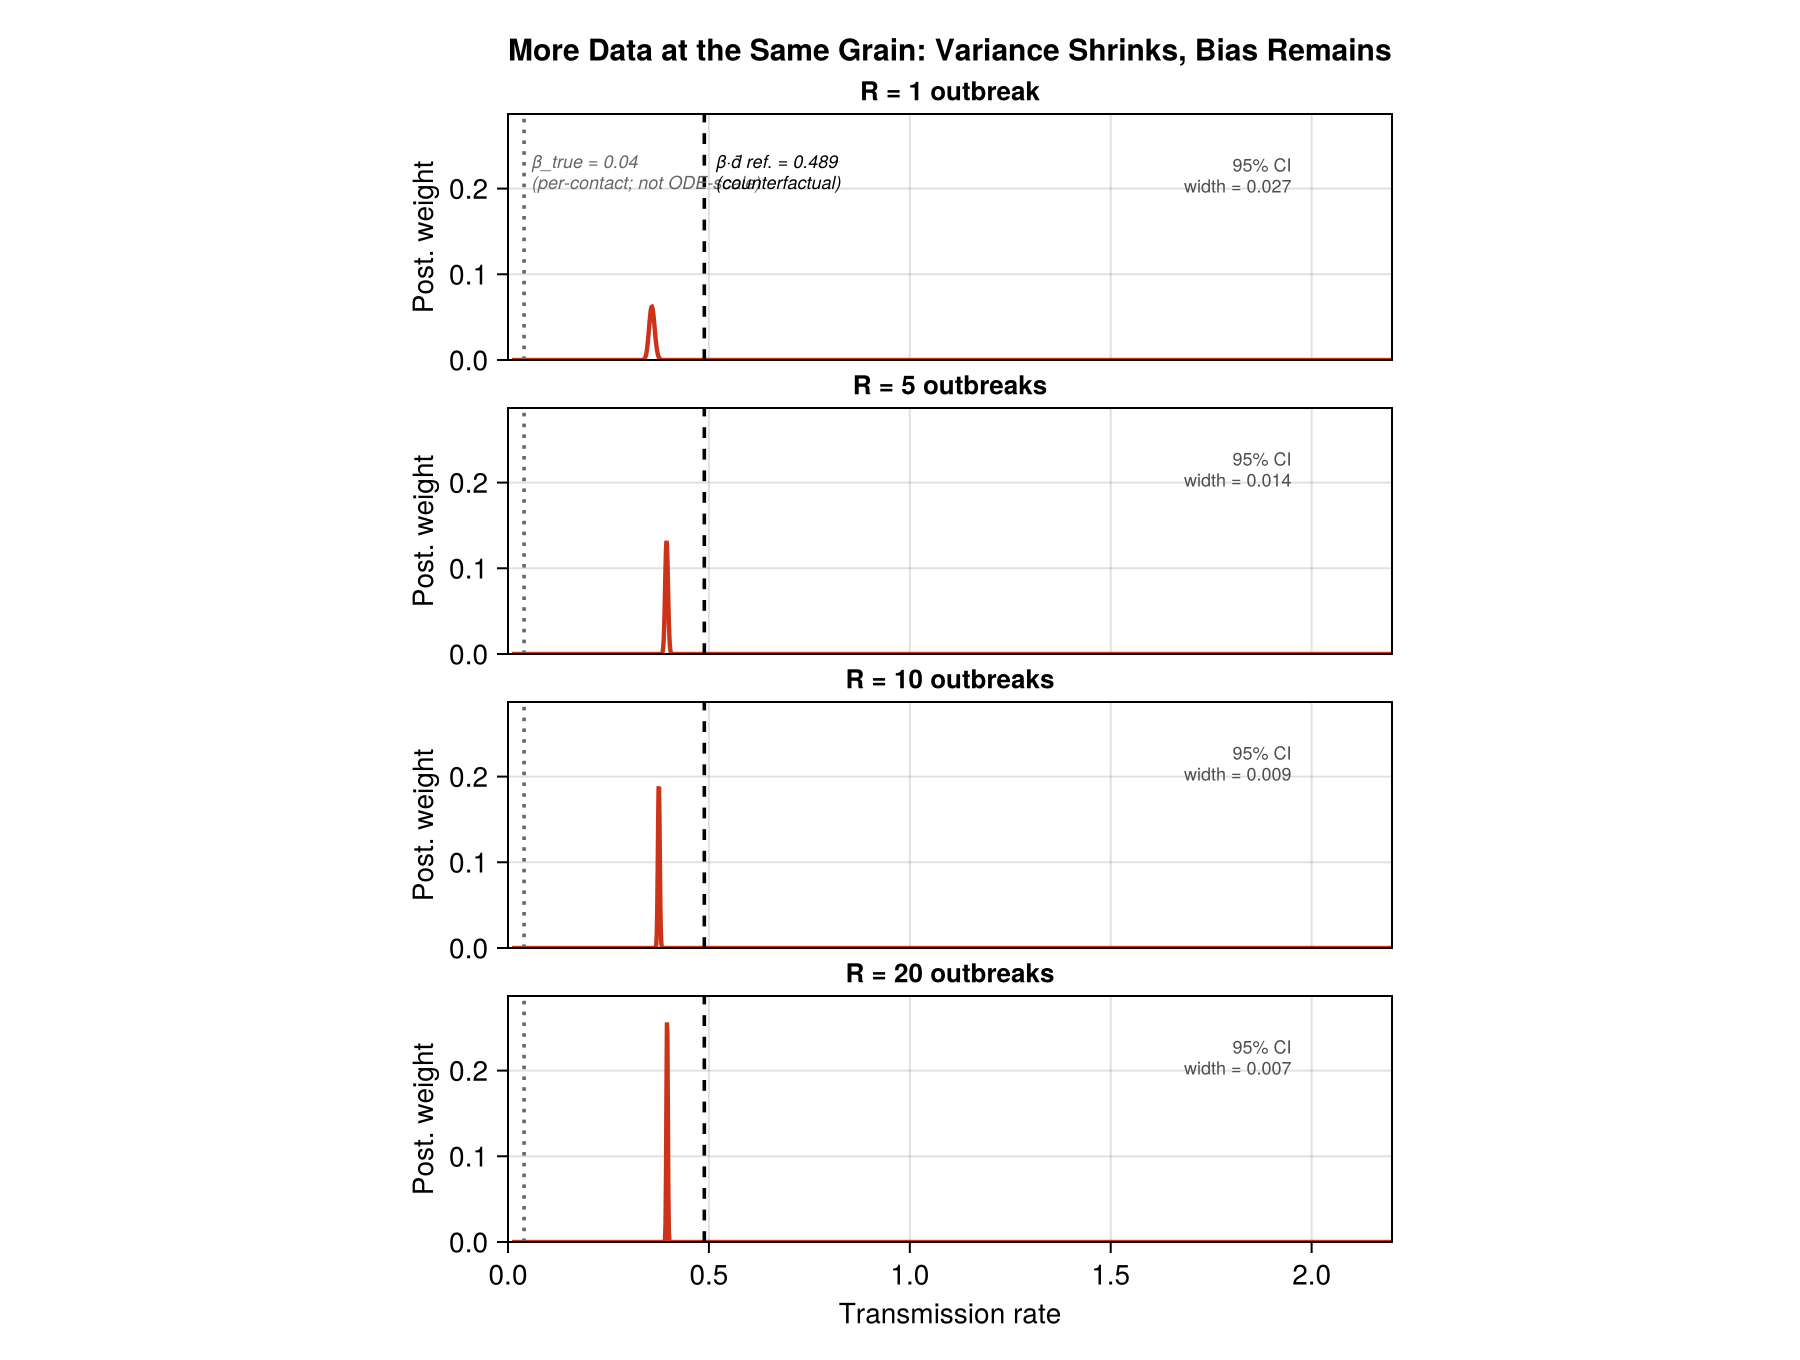
\includegraphics[width=0.82\linewidth]{../figures/fig_04_more_data_shrinks_variance_not_bias.png}
  \caption{Pooling $R=1,5,10,20$ weekly aggregate outbreaks narrows the ODE
    posterior nearly fourfold without moving it to the density-matched reference
    (dashed). Repetition at the same grain and clock sharpens the reduced model.}
  \label{fig:more_data}
\end{figure}


\section{Network Uncertainty and PAC-Bayesian Regularization}

We quantify uncertainty in $\eta$ under each observation process and prior. For
incidence observations, we estimate a simulation-based synthetic likelihood from
20 replicated epidemics per grid point and evaluate it on 30 independent held-out
epidemics generated under both a uniform network ($\eta=0$) and a structured
network ($\eta=2.5$). The prior comparison makes the intended tradeoff explicit.
Under the uniform generator, a moderate spike-and-slab prior leaves less posterior
mass on spurious structure than a moderate half-normal prior; for group-weekly
data, the corresponding mass above $\eta=0.25$ is $0.27$ versus $0.58$. Under the
structured generator, the same conservative prior increases downward bias: the
mean group-weekly posterior for $\eta$ is $1.32$ under spike-and-slab and $1.50$
under half-normal. Aggregate observations are shrunk still more strongly. This is
the desired behavior: when grain and clock provide weak evidence about topology,
we accept conservative bias rather than confidently hallucinating structure.

\begin{figure}[htbp]
  \centering
  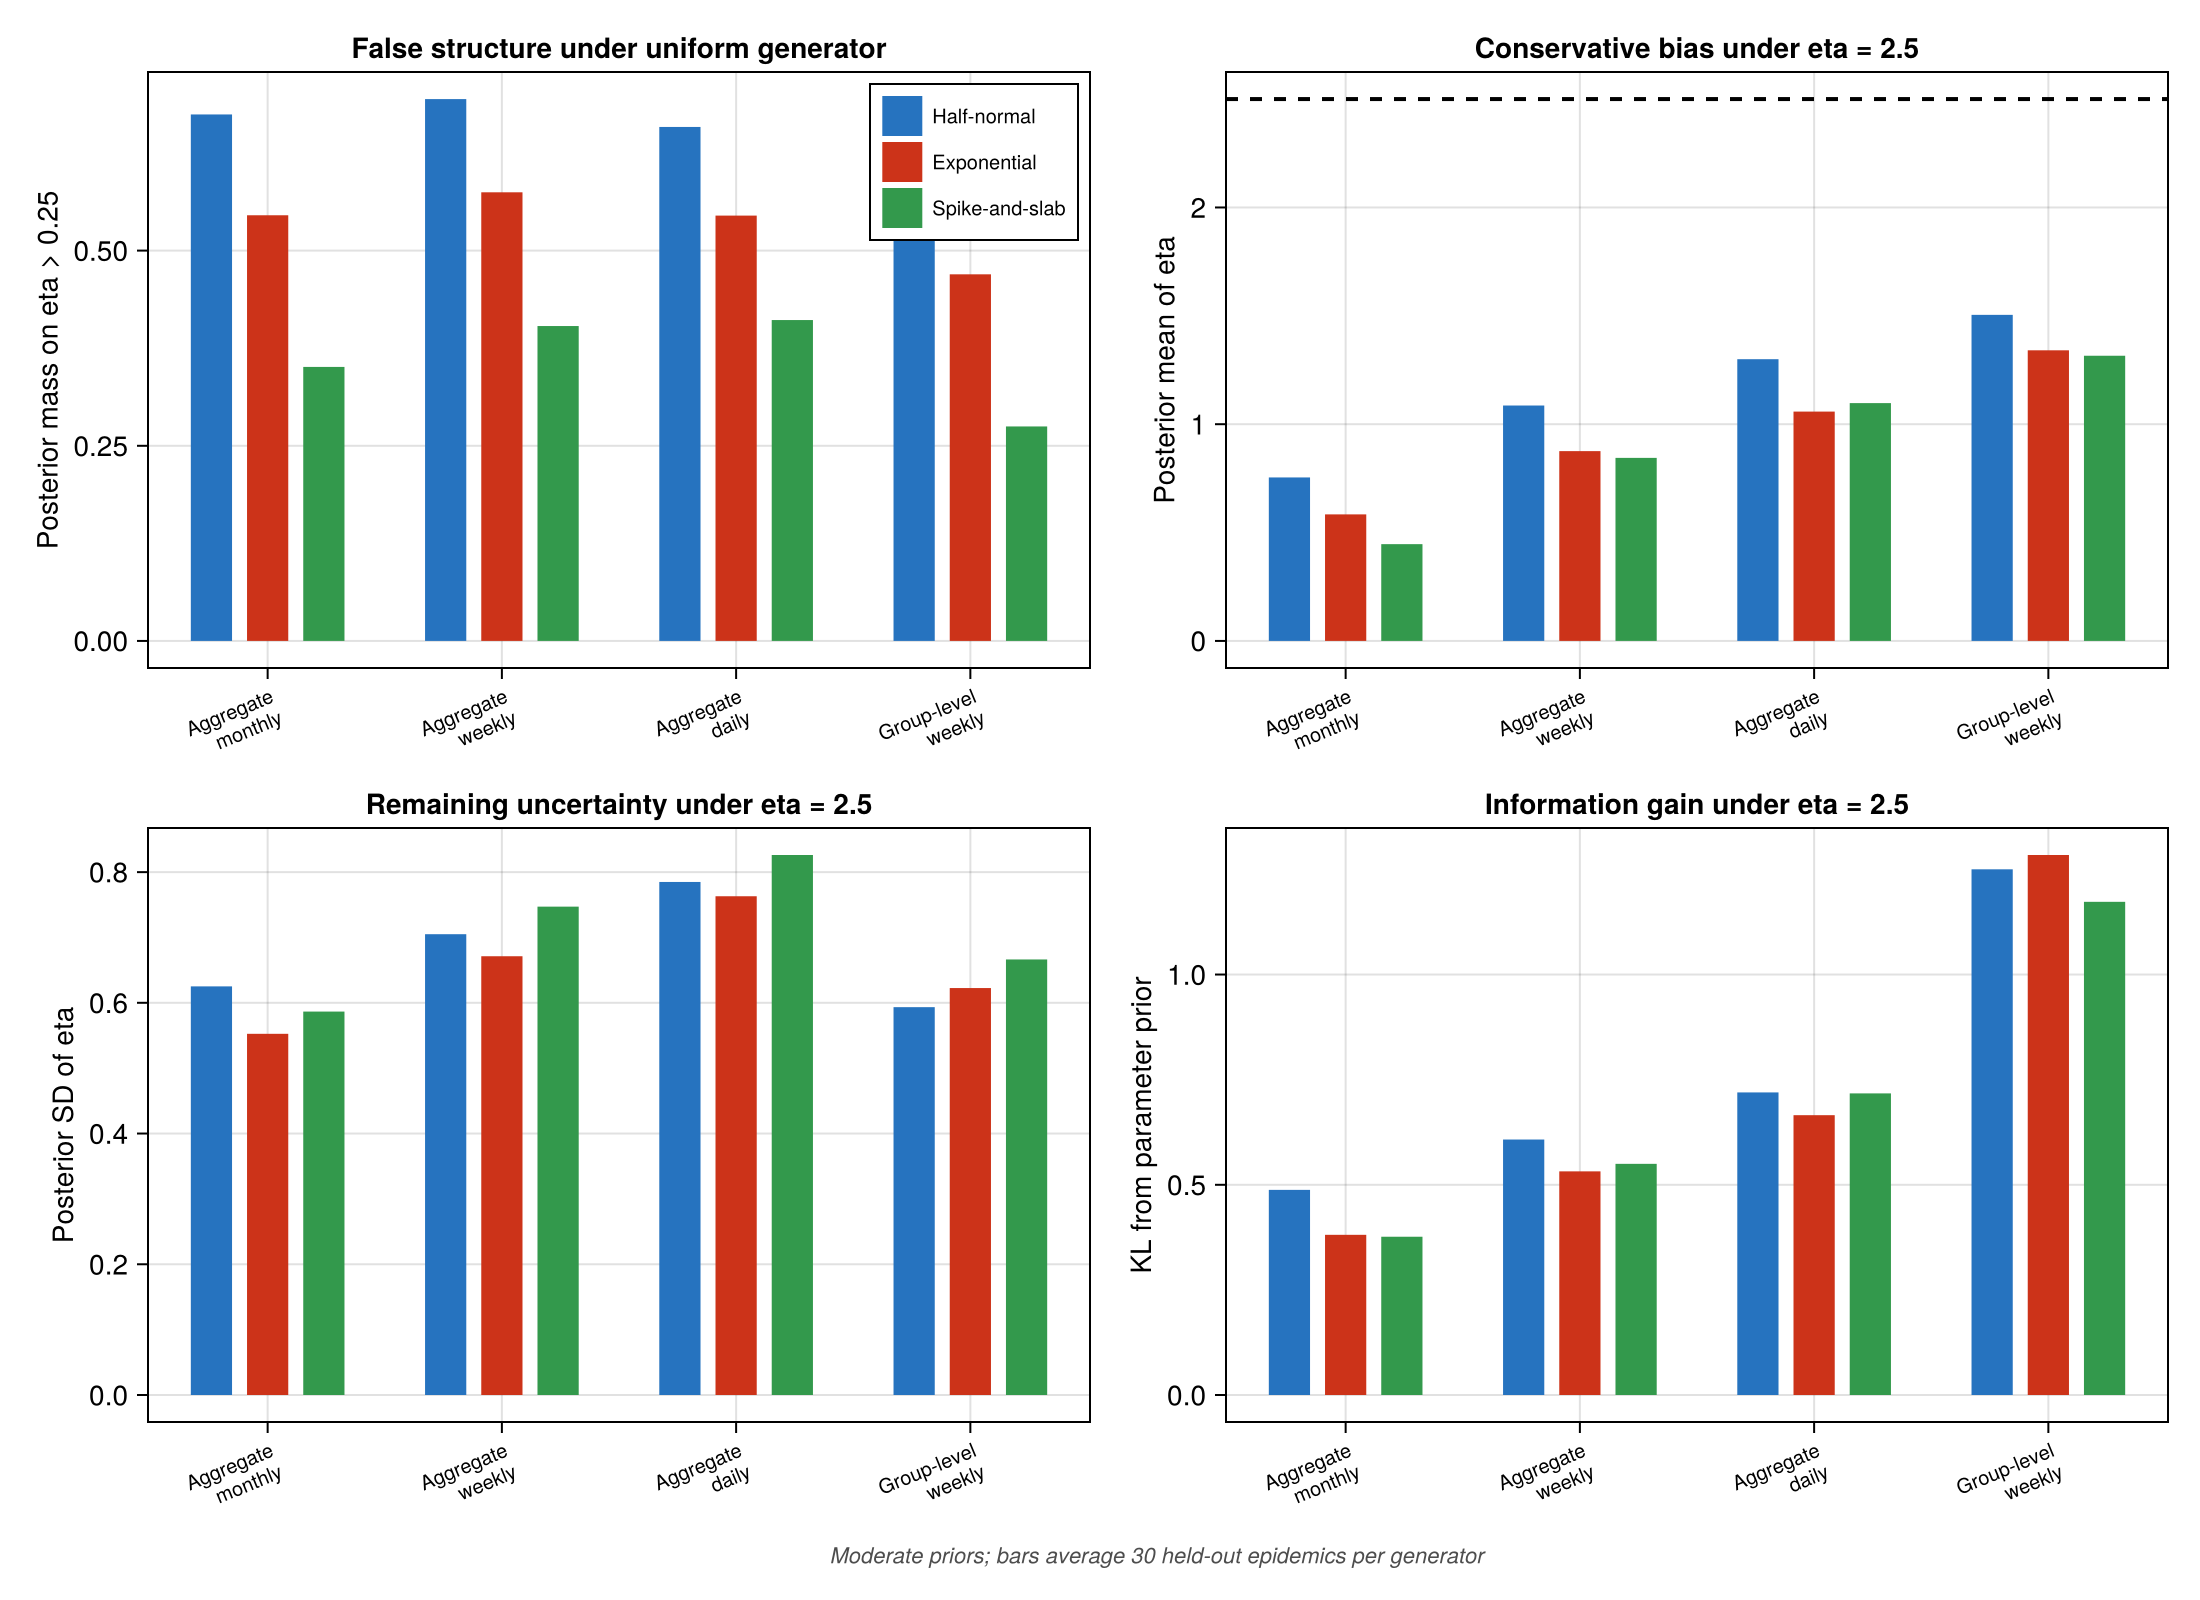
\includegraphics[width=0.90\linewidth]{../figures/fig_08_network_uq_by_observation.png}
  \caption{Prior sensitivity and observation-conditioned network uncertainty for
    moderate half-normal, exponential, and spike-and-slab priors. Top left: false
    structural mass under a uniform generator. Top right: shrinkage of the posterior
    mean under a structured generator ($\eta=2.5$, dashed reference). Bottom:
    posterior spread and information gain under the structured generator. Stronger
    concentration near uniformity suppresses invented structure at the cost of
    conservative bias when structure is present. Bars average 30 held-out epidemics.}
  \label{fig:network_uq}
\end{figure}

In a PAC-Bayesian formulation \citep{mcallester1999}, candidate network structures
or network-generating parameters are evaluated by predictive performance penalized
by departure from a prior over simpler or more regular mechanisms. Under rich
observation---such as contact edges or exposure histories---the posterior can move
substantially away from the regularizing prior. Under coarse observation---such as
weekly aggregate incidence---many network configurations can retain posterior mass.
For observation operator $\mathcal O_{g,c}$ and its associated calibration loss,
the generalized posterior takes the form
\[
 Q_{g,c}(d\eta) \propto
 \exp\{-\tau\widehat L_{g,c}(\eta)\}\,P(d\eta),
 \qquad A\mid\eta\sim P(A\mid\eta).
\]
Equivalently, $Q_{g,c}$ trades posterior-averaged predictive loss against
$\operatorname{KL}(Q_{g,c}\|P)$. Grain and clock therefore enter the loss through
the observation operator, while the parameter prior determines how unsupported
network structure is regularized.

PAC-Bayes offers a framework for quantifying which network distinctions the data
support and how uncertain unsupported distinctions should remain. This is the
appropriate inferential logic for
agent-based models: retain heterogeneity when the data support it, penalize it
when they do not, and quantify uncertainty when the observation process cannot
decide. A mechanism cannot be validated at a resolution where its identifying
information has been discarded. More data help only when they add information
relevant to the mechanism, not merely more replications of the same reduced
observation.

This framing clarifies the role of priors. A prior is a form of regularization:
it encodes which model configurations are penalized in the absence of data support,
exactly as a penalty term shrinks parameters toward a simpler structure
\citep{tibshirani1996}. Priors and perturbation schemes are in this sense
dual---both express assumptions about which departures from a baseline model should
require justification from the data \citep{hazan2016}.
The practical consequence is that disputes over which prior is \emph{correct} are
largely unproductive. No prior is uniquely correct; each encodes a different
regularization. What is productive is comparing priors: if conclusions are stable
across a range of reasonable priors, they are robust to that modeling choice. If
they are not, the instability is itself informative about what the data can and
cannot identify \citep{gelman2013}.

A practical workflow follows: (1)~specify the latent process and observation
process separately; (2)~place a regularizing prior over network structure;
(3)~condition that distribution under alternative grains and clocks; (4)~compare
posterior entropy, spread, and information gain; (5)~propagate network uncertainty
to epidemic and intervention predictions; (6)~run posterior predictive checks.

\section{Conclusion}

Mean-field SIR is not wrong because it is mathematically crude; it is wrong because
it encodes a social theory of uniform contact. Whether that wrongness matters
empirically depends on the observation process. The inferential target should be a
distribution over compatible networks whose uncertainty is explicitly conditional
on observational grain and clock. Regularized network inference retains
heterogeneity when observations constrain it and preserves uncertainty when they do
not.

Under weekly aggregate incidence, additional outbreaks reduce posterior variance
around a pseudo-true ODE parameter but do not recover the network mechanism. More
data at the same grain and clock estimate the wrong reduced model more precisely.
The fully qualified claim is this: more data make the wrong model more certain when
the additional data are collected under the same insufficient observation process.
Direct contact-network observation sharply reduces uncertainty about community
structure in our experiment. Group-level incidence produces a smaller but meaningful
update, while finer aggregate timing alone yields limited information about topology.
The point is not to declare one network recovered or unrecovered, but to quantify
the distribution of networks compatible with each observation process. Coarse data
require regularized uncertainty rather than false mechanistic confidence.

\bibliographystyle{plainnat}
\bibliography{references}

\end{document}
